\documentclass[12pt,letterpaper,ngerman]{article}
%\usepackage[letterpaper,top=3.0cm, bottom=3.0cm, footnotesep=1.0cm]{geometry}
\usepackage[letterpaper,margin=1in]{geometry} % e. Set margins of 1 inch (2.54 cm.) on all four sides of the paper. 
\usepackage{mathptmx} % d. ...in a simple roman face except where indicated below (§3). 
\usepackage[singlespacing]{setspace} % Set line spacing to 1 throughout the document
\usepackage{fancyhdr} 

% Set the headheight to at least 14.49998pt
\setlength{\headheight}{14.49998pt}

% Optionally adjust \topmargin if necessary
% \addtolength{\topmargin}{-2.49998pt}
\usepackage{relsize}

\usepackage[bottom]{footmisc}
\usepackage{tabularx}
    
\pagestyle{empty}        % No page numbers

% Set paragraph indentation to 1.5cm
\setlength{\parindent}{2em}

%%%Using XeTeX (xelatex, lulatex):
%\usepackage{polyglossia}
%\usepackage{fontspec}
%\usepackage{xunicode}
%\usepackage{xltxtra}
\usepackage{url}
\usepackage{hyperref}
\usepackage[english,german]{babel}

\usepackage{graphicx}

%\setmainfont[Mapping=tex-text]{Linux Libertine O} %Falls nicht vorhanden müssen die LinLibertine-ttf-Dateien nach C:\windows\fonts verschoben werden

\usepackage{booktabs}    % For nice-looking tables
\usepackage{natbib}      % Citation support (required for crossrefs)
\usepackage{expex}
\bibpunct[:]{(}{)}{;}{a}{}{,} % Defaults for in-text citations
\usepackage{bibentry}    % Print individual references

\usepackage{acronym}
\usepackage{multicol}

% TODO: set authors name
%vorgelegt von\\
%Name des Verfassers/der Verfasserin\\
\author{Author's name}

\usepackage{scrhack} % Recommended to avoid potential conflicts
\usepackage{microtype}

\usepackage[acronym,xindy,toc]{glossaries} % TODO: include "acronym" if glossary and acronym should be separated
\makeglossaries
\loadglsentries{pages/glossary.tex} % important update for glossaries, before document

\usepackage{ragged2e}

% Set up hyphenation rules for the language package when mistakes happen
\babelhyphenation[english]{
an-oth-er
ex-am-ple
}

\usepackage{babel}
\usepackage{csquotes}
\MakeOuterQuote{"}
\usepackage{mathtools}
\usepackage{amssymb}
\usepackage{amsmath}
\usepackage{tikz}
\usepackage{chngcntr}
\usepackage{float}
\usepackage{svg}
\usepackage{cite}
\usetikzlibrary{
  decorations.pathmorphing,
  automata, positioning, arrows, matrix,
  decorations.pathreplacing,
  shapes.geometric, calc,shapes.misc,
  arrows.meta,backgrounds,fit,petri
}
\pgfmathsetseed{\number\pdfrandomseed} % to ensure that it is randomized
\begin{document}
\DeclarePairedDelimiter\ceil{\lceil}{\rceil}
\DeclarePairedDelimiter\floor{\lfloor}{\rfloor}
\newcommand{\rand}[2]{
\pgfmathsetmacro{\thenum}{rand(0,1)}
\thenum
}
\newcommand{\nat}[0]{\mathbf{N}}
\newtheorem{example}{Beispiel}[section]


\begin{center}\uppercase{Ludwig-Maximilians-Universität München}\end{center}
\begin{center}
  \uppercase{Programming languages and artificial intelligence}
\end{center}

\vspace*{10mm}
\begin{center}

\includegraphics[height=40mm]{abb/sigillum.png}
\end{center}
\vspace*{10mm}

\title{Titel der Arbeit}
\date{\vspace{-5ex}}
{\let\newpage\relax\maketitle}
\thispagestyle{empty}
\begin{center}
\begin{large}
\begin{Large}
Bachelorarbeit\\
\end{Large}
im Studiengang 'Informatik plus Mathematik' \\
\end{large}
\end{center}
\vspace{1cm}
\begin{center}
\begin{large}
Betreuer: Prof. Dr. Johannes Kinder\\
\end{large}
\end{center}
\begin{center}
\begin{large}
Mentor: Moritz Dannehl, M.Sc.\\
\end{large}
\end{center}


\begin{center}
\begin{large}
Ablieferungstermin: \date{\today} \\
\end{large}
\end{center}

\vspace{1,5cm}

\newpage
\tableofcontents
\newpage

\setcounter{page}{1}
\pagestyle{fancy}
\fancyhf{}
\counterwithin{figure}{section}
\fancyhead[R]{\thepage}
\renewcommand{\headrulewidth}{0pt} %obere Trennlinie
\newtheorem{definition}{Definition}
\section*{Abstract}
\section{Einführung}
In den letzten Jahren wurden wichtige Fortschritte in der natürlichen
Sprachverarbeitung erzielt, ein wichtiger Faktor war die Codierung von
natürlicher Sprache in reellwertigen Vektoren (engl. embeddings). Die hochdimensionalen Vektoren
codieren die Semantik der ursprünglichen Wörter oder Sätze. Die daraus 
resultierenden Vektoren erlauben es, neuronale Netzwerke in diversen 
Anwendungsbereichen zu trainieren, wie beispielsweise. 
\textit{spam detection} \cite{Ball2019}.  
Zu den bekanntesten Modellen, die natürliche Sprache in Vektoren abbilden, gehören 
\textit{Word2Vec} \cite{mikolov2013efficientestimationwordrepresentations},
\textit{WordPiece} \cite{wu2016googlesneuralmachinetranslation} und
\textit{SentenceTransformer} \cite{reimers2019sentencebertsentenceembeddingsusing}.\\

Diese Fortschritte dienen als Motivation, auch Assembler Quellcode auf einen 
Vektor abzubilden, der die Semantik des Quellcodes codiert. Die resultierenden
Vektoren können dann wieder benutzt werden, um neuronale Netzwerke auf
diverse Anwendungen zu trainieren, wie beispielsweise
\textit{binary code similarity detection} \cite{wang2022jtransjumpawaretransformerbinary},
\textit{function boundary detection} \cite{190918},
\textit{function type inference}\cite{203650},
\textit{binary code search} \cite{9345532},
Reverse Engineering \cite{lacomis2019direneuralapproachdecompiled},
oder das Klassifizieren von 
Malware in der Maschinensprache\cite{raff2017malwaredetectioneatingexe}.\\

Um ein Modell mittels überwachtes Lernen zu trainieren, das Assemblercode in 
semantische Vektoren abbildet, ist für jede Assembler-Funktion ein Vektor 
erforderlich, der die Semantik der Funktion codiert. Der Datensatz kann durch 
Kompilieren des Quellcodes von höheren Programmiersprachen generiert 
werden.\\

\textit{Ziel}: Das Ziel dieser Arbeit ist es, verschiedene Methoden zu vergleichen
aus C Quellcode Vektoren zu generieren, die die Semantik von dem ursprünglichen
Quellcode codieren, mithilfe von Werkzeugen aus der natürlichen Sprachverarbeitung.\\

\textit{Motviation}: Der Prozess des Kompilierens reduziert Funktionen
auf die für den Computer wesentlichsten Bausteine, dabei gehen viele 
Informationen verloren, wie Funktionsnamen, Variablennamen und Kommentare. 
Diese Informationen sind von großer Bedeutung und geben Aufschluss über 
die Funktionsweise und den Anwendungszweck der Funktion. Durch die Verwendung 
dieser Informationen könnte die semantische Codierung des Quellcodes verbessert
werden. Aufgrund der Tatsache, dass diese Informationen in der natürlichen 
Sprache sind, ist es sinnvoll, bewährte Werkzeuge aus der natürlichen 
Sprachverarbeitung zu verwenden, um diese in semantische Vektoren zu codieren. 
Aus den resultierenden Vektoren kann schließlich ein Datensatz generiert werden,
der ein neuronales Netzwerk darauf trainiert, Assemblercode auf hochdimensionale,
reellwertige Vektoren abzubilden, die die Semantik des Quellcodes codieren.
\pagebreak
\subsection{Stand der Technik}
Das {\bf CLAP} ({\bf C}ontrastive {\bf L}anguage {\bf A}ssembly {\bf P}re-training) 
Paper \cite{wang2024claplearningtransferablebinary} 
setze Anfang 2024 einen neuen Stand der Technik, mithilfe von natürlicher
Sprachverarbeitung, in \textit{binary code simillarity detection}. Die Aufgabe 
besteht dabei darin, die semantische Ähnlichkeit zwischen zwei gegebenen 
Assemblercodes zu bestimmen.\\

Das Clap-Modell ist aus zwei Teilen zusammengesetzt: einem Assembler-Encoder 
und einem Text-Encoder. Der Assembler-Encoder, der aus Assemblercode 
reellwertige Vektoren erzeugt, knüpft mit kleinen Änderungen an den vorherigen
Stand der Technik von JTrans an. Der Text-Encoder ist eine völlig neue Idee, 
die darauf abzielt, den Text wieder in einen reellwertigen Vektor zu 
konvertieren. Wang et. al starten dabei mit einem Modell aus der natürlichen 
Sprachverarbeitung namens \textit{SentenceTransformer} und trainieren dieses
darauf, Assemblercode die passende Quellcodeerklärung  zuzuordnen. Dabei 
erhalten sie die Quellcodeerklärungen durch ein Large  Language Model, wie
beispielsweise Chat-GPT.\\

Das {\bf JTrans}-Modell \cite{wang2022jtransjumpawaretransformerbinary}
baut auf einer Modellarchitektur aus der natürlichen 
Sprachverarbeitung namens 
Transformer \cite{vaswani2023attentionneed} auf. 
Wang et. al behandeln die einzelnen Assembler-Instruktionen als Wörter, um so 
die Transformer Modellarchitektur anwenden zu können. Außerdem codieren sie
Kontrollflussinformationen des Assemblercodes in die Eingabe des 
Transformer-Modells. Mit diesem Ansatz erzielten sie im Jahre 2022 einen neuen
Stand der Technik in \textit{binary code similarity detection}.

\subsection{Leistungen der Arbeit}
Die hauptsächlichen Leistungen dieser Arbeit sind:
\begin{itemize}
  \item Ein Tool, das einen Datensatz mit Assemblercode und semantischen 
    Vektoren aus C-Quellcode und dem dazugehörigen Assemblercode generiert.
  \item Eine qualitative Analyse durch 
    \textit{t-SNE} \cite{JMLR:v9:vandermaaten08a}, die die Verwendung von 
    Funktionskommentaren, Funktionsnamen, 
    \textit{Code Llama} \cite{rozière2024codellamaopenfoundation} Erklärungen
    und \textit{Code2Vec} \cite{alon2018code2veclearningdistributedrepresentations}
    untersucht.
  \item Eine quantitative Auswertung, die durch Befragung von Experten erfolgt,
    vergleicht die Verwendung von Funktionsnamen, \textit{Code Llama} 
    Erklärungen und \textit{Code2Vec} miteinander.
  \item Eine Formel, die die Verwendung von Funktionsnamen, \textit{Code Llama}
    Erklärungen und \textit{Code2Vec} vergleicht.
\end{itemize}
\pagebreak
\subsection{Aufbau der Arbeit}
Kapitel 2 führt anfangs grundlegende Konzepte und Begriffe des maschinellen 
Lernens ein. Anschließend werden semantische Vektorräume in Bezug auf 
natürliche Sprache erläutert und die größten Fortschritte der letzten Jahre 
beschrieben. Am Ende werden noch \textit{Code Llama}, \textit{Code2Vec} und 
\textit{t-SNE} vorgestellt, welche eine wichtige Rolle in dieser Arbeit spielen.\\

Die allgemeine Architektur des Tools und dessen Designentscheidungen werden im Kapitel 3
beschrieben. Es werden die Auswahl des C-Quellcodes, die Datenpipeline und die 
Stabilität des \textit{SentenceTransformers} erläutert.\\

Kapitel 4, 5, 6 und 7 befassen sich mit den verschiedenen Methoden, Embeddings
zu erzeugen. Also wie aus den Quellcodeinformationen über Funktionsnamen und
-kommentare ein Vektor erstellt werden kann. Außerdem wird erläutert, wie mit
\textit{Code Llama} und \textit{Code2Vec} Vektoren produziert werden können.\\

Die Ergebnisse werden in einer qualitativen und quantitativen Auswertung in 
Kapitel 8 vorgestellt. Zuerst wird durch eine Experten-Evaluierung die beste
Methode identifiziert. Anhand dieser Einordnung wird überprüft, ob die Formel
und Analyse durch \textit{t-SNE} ein ähnliches Ergebnis aufweisen.\\

Die Ergebnisse werden im Kapitel 9 reflektiert, eingeordnet und diskutiert. 
Es werden die Stärken und Schwächen jeder Methode dargestellt und diskutiert.\\

Im letzten Kapitel wird die gesamte Arbeit reflektiert und anschließend ein 
Ausblick gegeben, um weitere Anregungen für die weitere Arbeit in diesem Thema
zu geben.

\pagebreak
\section{Grundlagen und Termini}
\subsection{Maschienelles Lernen}
Heutzutage ist maschinelles Lernen weitverbreitet und wird in nahezu jedem
Bereich der Informatik verwendet.  Maschinelles Lernen wird überall dort 
eingesetzt, wo eine analytische Lösung eines Problems zu aufwendig oder gar 
überhaupt nicht existiert. Maschinelles Lernen sucht nach einer Lösung, indem 
es aus den Daten ein Muster ableitet. Sind die Daten endlich, ist meist das 
resultierende Modell nur eine Approximation der gesuchten Lösung. In diesem 
Abschnitt wird zunächst maschinelles Lernen definiert und dann darauf aufbauend 
grundlegende Trainingsarten vorgestellt.
 % Book: Learingin from data, page 1, row 6
\subsubsection{Definition}
Die weit verbreitete Ansicht, dass maschinelles Lernen nur etwas mit neuronalen 
Netzwerken zu tun hat, ist im Allgemeinen falsch. Generell kann ein Problem, 
das mit maschinellem Lernen gelöst wird, wie folgt definiert werden:
\begin{definition}
  Sei $X$ eine beliebige Input Menge, $Y$ eine beliebige Output Menge,
  $f \in \{X \to Y\}$ die gesuchte Lösung des Problems, 
  $\mathbb{D}$ eine beliebige Menge aus gegebenen Datenpunkten,\\
  $H_1 \subset \{X \to Y\}$ ein Hypothesenraum, und 
  $A_1: \mathcal{P}(\{X \to Y\}) \times 
  \mathcal{P}(\mathbb{D}) \to \{ X \to Y \} $
  ein Lernalgorithmus. Dann ist das ziel, bei gegebenen Daten,
  den Hypothesenraum $H_1$ und den Lernalgorithmus $A_1$ so zu wählen,
  sodass
  \[
    A_1(H_1, \mathbb{D}) \approx f.
  \]
\end{definition}
Maschinelles Lernen ist also die Suche nach einem Lernalgorithmus und 
Hypothesenraum, der dann in Kombination mit gegebenen Daten die bestmögliche
Lösung approximiert. Dabei ist hervorzuheben, dass der Datensatz das Herzstück
jeder Problemstellung im Bereich des maschinellen Lernens ist. Wenn der
Datensatz zu klein oder überhaupt nicht repräsentativ für das gegebene Problem 
ist, wird der Lernalgorithmus die falschen Muster erkennen und dadurch eine 
fehlerhafte Approximation erzeugen.
\begin{figure}[H]
  \begin{center}
    \begin{tikzpicture}
    [inner sep=2mm,
     place/.style={circle,draw=blue!50,fill=blue!20,thick},
     transition/.style={rectangle,draw=black!50,fill=black!20,thick}]
    \node (F) at (-1,4) [transition] {Lösung  $f: X \to Y$};
    \node (D) at (-1,2) [transition] {Datenpunkte $\mathbb{D}$};
    \node (H) at (-1,0) [transition] {Hypothesenraum $H_1$};
    \node (A) at (3,1) [place, label=Lernalgortihmus] {$A_1$};
    \node (FH) at (6,1) [transition, label=Approximation] {$g \approx f$};
    \draw [->] (H) .. controls +(up:8mm) and +(left:8mm)
                         .. (A)
               (D) .. controls +(down:8mm) and +(left:8mm)
                         .. (A);
    \draw[->] (A) -- (FH);
      \draw [->,decorate,
       decoration={snake,amplitude=.4mm,segment length=2mm,post length=1mm}]
      (F) -- (D);
    \end{tikzpicture}
    \caption{Grundlegendes maschinelles Lernen Problem}
  \end{center}
\end{figure}
\pagebreak
In der Figur 2.1 ist die Problembeschreibung noch einmal bildlich dargestellt.
Beachtenswert ist, dass die Datenpunkte nicht immer in Abhängigkeit mit 
$f: X \to Y$ stehen. Beispielsweise können die Datenpunkte einfach nur aus den
Eingabewerten bestehen: $\mathbb{D} = \{x_1,x_2,x_2, \dots, x_n\} \subset X$.
Die Struktur des Datensatzes kann sehr unterschiedlich sein, das hängt auch mit 
unterschiedlichen Lernmethoden zusammen.
\subsubsection{Deep-Learning}
Vor der Betrachtung der Lernmethoden wird kurz auf Deep Learning eingegangen.
Deep Learning ist ein neuronales Netzwerk, das über mehrere Layer zwischen
Input und Output Layer verfügt. 
Zunächst einmal müssen wir neuronale Netzwerke definieren, die folgende
Definition ist inspiriert aus der Vorlesung Computational Intelligence
der LMU München:
\begin{definition}
  Ein neuronales Netzwerk (NN) ist eine Funtion $N: \mathbb{R}^q \to \mathbb{R}^p$,
  wobei $q\in \mathbb{N}$ die Anzahl der Inputs und $p \in \mathbb{N}$ die
  Anzahl der Outputs ist. Sei $(L_i)_{i \in \{ 1, \dots, n\}}$ die Layer,
  $(K_i^l)_{l=1,\dots, n, i = 1,\dots r_l}$ die Konten im jeweiligen Layer 
  $l \in \{1, \dots, n\}$ und $r_l \in \mathbb{N}$ die Anzahl der Knoten im
  Layer $L_l$. Jeder Koten im Layer $L_l$ ist mit jedem Knoten im 
  Layer $L_{l+1}$ verbunden, mit $l \in \{1,\dots, n-1\}$. Jede Verbindung
  besitzt ein Gewicht $W_{i,j}^l$, wobei $l \in \{1,\dots, n-1\}$ und 
  das Gewicht der Verbindung $K^l_i \to K^{l+1}_j$ zugeordnet ist.
  Daraus ergibt sich eine Famillie von Matritzen 
  $(W_l)_{l=1,\dots, n-1}$, wobei $ W_l\in \mathbb{R}^{r_l\times r_{l+1}}$.
  Nun hat jeder Layer noch ein sogenannten Bias $(B_l)_{l = 2,\dots,n}$,
  dieser ist ein Zeilenvektor $B_l \in \mathbb{R}^{r_l}$.
  Als letztes braucht jeder Knoten eine Aktivierungsfunktion, dass heißt
  für jeden Layer gibt es $r_l$ Funktionen:
  $(F_l)_{l=1,\dots,n}$, mit $F_l \in \{\mathbb{R} \to \mathbb{R}\}^{r_l}$.
  Es ist hilfreich die Funktionsanwendung auch für den Vektor $F_l$ zu definieren:
  Sei $x \in \mathbb{R}^{r_l}$, dann setze
  \[
    F_l(x) := \begin{pmatrix} 
        f_1(x_1) \\
        \vdots\\
        f_{r_l}(x_{r_l})
    \end{pmatrix}.
  \]
  Dann ist die Funktion $N: \mathbb{R}^q \to \mathbb{R}^p$ wie folgt definiert:
  %\[
  % N(x) = F_n(W_nf_{n-1}(W_{n-1} \dots f_1(W_1) \dots ))
  %\]
  \[
    N(x) = h_1(x)
  \]
  ,wobei
  \[h_l: \mathbb{R}^{r_l} \to \mathbb{R}^{r_l+1}\]
  \[
    h_l(x) = 
      \begin{cases}
        h_{l+1}(F_{l+1}(W_lx + B_{l+1}))& ,  \text{if } l < n \\ 
        x & , \text{sonst}\\
      \end{cases}.
  \]
  Wir bezeichnen $L_1$ als Input-Layer, $L_n$ als Output-Layer und
  $L_i$, mit $i \in \{2, \dots, n-1\}$, als Hidden-Layer.
\end{definition}
Deep Learning ist ein Hypothesenraum, da alle neuronalen Netzwerke 
höherdimensionale reellwertige Funktionen sind. Schließlich gilt für den
Hypothesenraum:
\[
  H = \{\mathbb{R}^n \to \mathbb{R}^k\}, \text{ wobei } n,k \in \mathbb{N}
\]
Die Definition von einem Neuronalen Netzwerk erscheint zunächst länglich und unintuitiv, diese
wird aber anschaulich anhand eines Beispiels.
\begin{example}
  Sei $N: \mathbb{R}^2 \to \mathbb{R}^2$, $(L_i)_{i=1,2,3}$ Layer.
  Der Input-Layer besitzt zwei Knoten $r_1 = 2$, der erste
  Hidden-Layer besitzt $r_2 = 3$, der zweite Hidden-Layer besitzt
  $r_3 = 3$ Knoten und der Output-Layer besitzt $r_4 = 2$ Knoten.
  Mit den Knoten $(K^l_i)_{l=1,2,3, i = 1, \dots, r_l}$ und zufälligen
  Gewichten:
  \[
    W_1 = \begin{pmatrix} 0.2 & 0.7 & 0.4 \\ 0 & 0.7 & 0.8 \end{pmatrix} 
    \in \mathbb{R}^{2 \times 3},
    W_2 = \begin{pmatrix} 0.6 & 0 & 0.4 \\ 0.1 & 0.7 & 0.8 \\ 1 & 0.33 & 0.2 \end{pmatrix}
    \in \mathbb{R}^{3 \times 3},
    W_3 = \begin{pmatrix} 0.2 & 0.45 \\ 0.1 & 0.23 \\ 1 & 0.33 \end{pmatrix}
    \in \mathbb{R}^{3 \times 2}.
  \]
  Für den Bias setzen wir:
  \[
    B_2 = \begin{pmatrix} 0.1 \\ 0.2 \\ 0.3\end{pmatrix} \in \mathbb{R}^3,
    B_3 = \begin{pmatrix} 0.4 \\ 0.5 \\ 0.6\end{pmatrix} \in \mathbb{R}^3,
    B_4 = \begin{pmatrix} 0.7 \\ 0.8 \end{pmatrix} \in \mathbb{R}^2,
  \]
  Außerdem setzen wir alle Aktivierungfunktionen:
  \[
    (F_{l})_i = \text{tanh}, \text{ wobei } l \in \{ 1, 2, 3\},
      i \in \{1, \dots, r_l\}
  \]
  Dann gilt für das Neuronales Netzwerk $N: \mathbb{R}^2 \to \mathbb{R}^2$:
  \[
    N(x) = 
    {\color{green}
    \text{tanh}(\begin{pmatrix} 0.2 & 0.45 \\ 0.1 & 0.23 \\ 1 & 0.33 \end{pmatrix}
    }
    {\color{blue}
    \text{tanh}(\begin{pmatrix} 0.6 & 0 & 0.4 \\ 0.1 & 0.7 & 0.8 \\ 1 & 0.33 & 0.2 \end{pmatrix}
    }
    {\color{red}
    \text{tanh}(\begin{pmatrix} 0.2 & 0.7 & 0.4 \\ 0 & 0.7 & 0.8 \end{pmatrix}x
      + \begin{pmatrix} 0.1 \\ 0.2 \\ 0.3\end{pmatrix})} 
    {\color{blue}
      + 
    \begin{pmatrix} 0.4 \\ 0.5 \\ 0.6\end{pmatrix})}
    { \color{green}
    +
    \begin{pmatrix} 0.7 \\ 0.8 \end{pmatrix})
    }
  \]
  \begin{figure}[H]
    \begin{center}
      \begin{tikzpicture}
      [inner sep=2mm,
       place/.style={circle,draw=blue!50,fill=blue!20,thick},
       transition/.style={rectangle,draw=black!50,fill=black!20,thick}]
      \node (L11) at (-1,3) [place] {$K_1^1$};
      \node (L12) at (-1,1) [place] {$K_2^1$};

      \node (L21) at (2,4) [place] {$K_1^2$};
      \node (L22) at (2,2) [place] {$K_2^2$};
      \node (L23) at (2,0) [place] {$K_3^2$};

      \node (L31) at (5,4) [place] {$K_1^3$};
      \node (L32) at (5,2) [place] {$K_2^3$};
      \node (L33) at (5,0) [place] {$K_3^3$};

      \node (L41) at (8,3) [place] {$K_1^4$};
      \node (L42) at (8,1) [place] {$K_2^4$};

      \draw[->, red] (L11) -- (L21);
      \draw[->, red] (L11) -- (L22);
      \draw[->, red] (L11) -- (L23);
      \draw[->, red] (L12) -- (L21);
      \draw[->, red] (L12) -- (L22);
      \draw[->, red] (L12) -- (L23);

      \draw[->, blue] (L21) -- (L31);
      \draw[->, blue] (L21) -- (L32);
      \draw[->, blue] (L21) -- (L33);

      \draw[->, blue] (L22) -- (L31);
      \draw[->, blue] (L22) -- (L32);
      \draw[->, blue] (L22) -- (L33);

      \draw[->, blue] (L23) -- (L31);
      \draw[->, blue] (L23) -- (L32);
      \draw[->, blue] (L23) -- (L33);

      \draw[->, green] (L31) -- (L41);
      \draw[->, green] (L31) -- (L42);

      \draw[->, green] (L32) -- (L41);
      \draw[->, green] (L32) -- (L42);
        
      \draw[->, green] (L33) -- (L41);
      \draw[->, green] (L33) -- (L42);
      \end{tikzpicture}
      \caption{ Neuronales Netzwerk bildlich als Graph dargestellt}
    \end{center}
  \end{figure}
  Ein Gewicht zwischen zwei Knoten $K_1^1 \to K_1^2$ kann nun einfach nachgeschaut werden:
  \[
    (W_1)_{1,1} = 0.2
  \]
\end{example}
\pagebreak
In diesem Beispiel handelt es sich um Deep Learning, da das neuronale Netzwerk 
zwei Hidden-Layer besitzt. Deep Learning Models verfügen heutzutage über
eine zwei- bis dreistellige Anzahl an Hidden-Layer, diese Dimensionen sind 
aber für ein Beispiel ungeeignet.
\subsubsection{Überwachtes Lernen}
%learning from data page 11 row 7
Das überwachte Lernen ist die am häufigsten verwendete Trainingsmethode
und ist daher auch die wichtigste. Dieser Ansatz basiert immer auf der
korrekten Lösung für jeden Input und ist daher ein Tupel aus Input und
korrekten Outputwerten. 
  \[\mathbb{D} = \{ (x_1,y_1), (x_2,y_2) (x_3,y_3), \dots ,(x_n,y_n)\} 
  \subset X \times Y.\]
Ein Beispiel für diesen Ansatz ist die Bilderkennung, bei der ein Vektor
mit Grauwerten und ein ein Label bzw. eine Bezeichnung für das Bild
verwendet werden.
\begin{example}
  Sei $X = \mathbb{R}^{4096}$ und
   $Y = \{ \text{Katze}, \text{ Hund}, \text{ Auto}\}$, dann könnte der 
   Datensatz wie folgt aussehen:
   \[
     \mathbb{D} = \{
     (\begin{pmatrix} 0.2 \\ 0.9 \\ 0.5 \\ \vdots \end{pmatrix}, \text{Hund}),
     (\begin{pmatrix} 0.1 \\ 0.1 \\ 0.6 \\ \vdots \end{pmatrix}, \text{Hund}),
     (\begin{pmatrix} 0.6 \\ 0.7 \\ 0 \\ \vdots \end{pmatrix}, \text{Katze}),
     \dots, 
     (\begin{pmatrix} 0.4 \\ 0.3 \\ 0.9 \\ \vdots \end{pmatrix}, \text{Auto})
    \}
   \]
\end{example}
Der entscheidende Aspekt ist, dass wir das richtige Verhalten unseres Modells 
kennen und deshalb direkt wissen, wenn es Fehler macht. Beim selbst-überwachten
Lernen werden die richtigen Lösungen aus gegebenen Daten generiert. 
Bei vielen anderen Arten ist dieser Aspekt, der sehr natürlich erscheint,
nicht selbstverständlich.
\subsubsection{Unüberwachtes Lernen}
Das unüberwachte Lernen ist der Extremfall, da der Lernalgorithmus
ausschließlich die Inputwerte erhält.
\[\mathbb{D} = (x_1, x_2, x_3, \dots, x_n) \subset X\]
Der Lernalgorithmus erhält keine Hinweise darauf, was richtig oder falsch 
ist. Unüberwachtes Lernen ist eine Methode, um in Daten Strukturen und 
Muster zu identifizieren. Ein Beispiel ist die Cluster-Analyse, hier
bekommt der Lernalgorithmus eine Menge von Daten und gruppiert diese in
Teilmengen. In der Abbildung 2.3 ist ein Beispiel für das Resultat einer
möglichen Cluster-Analyse dargestellt.
\begin{figure}[H]
  \centering
  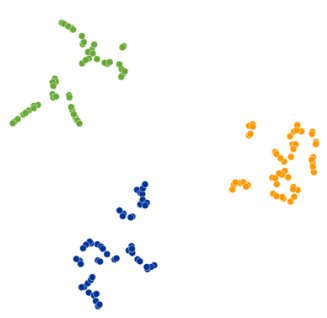
\includegraphics[scale=0.3]{abb/t-sne-example.png}
  \caption{Cluster Analyse angewendet auf 2-dimensionale Daten aus 
  \cite{wattenberg2016how}.}
\end{figure}

\subsubsection{Reinforcement Learning}
Das Reinforcement Learning ist nicht so extrem wie das unüberwachte Lernen. 
Bei diesem Paradigma liegen dem Lernalgorithmus zwar nicht die korrekten 
Outputwerte vor, aber der Lernalgorithmus erhält für jeden vorhergesagten Wert 
eine Rückmeldung, wie erwünscht dieser Wert ist. Ein Beispiel ist ein Modell,
das mittels eines Lernalgorithmus darauf trainiert wird, ein Videospiel zu 
gewinnen. Der Lernalgorithmus bekommt ein Abbild von der Umgebung und gibt dem 
Spiel einen Input, welcher eine Aktion zufolge hat. Falls nun die Aktion dazu 
beiträgt, den Spieler in eine gute Position zu bringen oder gar das Spiel zu
gewinnen, bekommt die Aktion eine positive Bewertung, andernfalls eine
negative. \\

Die Problemstellung im maschinellen Lernen ist allgemein formuliert und abstrakt.
Dies ist der Grund, warum maschinelles Lernen in vielen unterschiedlichen 
Bereichen eingesetzt werden kann. Einer der Bereiche ist die linguistische
Datenverarbeitung (engl. Natural Language Processing), was uns zum nächsten 
Begriff führt. Linguistische Datenverarbeitung wird im Folgenden mit NLP abgekürzt.

\subsection{Semantische Vekorräume}
Das semantische Codieren von natürlicher Sprache in einem Vektorraum 
ist ein bedeutsames Problem in NLP. %Referenz?
Der resultierende Vektorraum kann
für verschiedene Problemstellungen (engl. downstream tasks) verwendet
werden. Ein Beispiel ist die Klassifizierung von Spam-Nachrichten 
\cite{Ball2019}.
Semantischer Vektorraum heißt hier, dass ähnliche Wörter, also Wörter 
mit ähnlicher Bedeutung, im projizierten Vektorraum einen geringen 
Abstand zueinander haben. Wir werden die Vektoren im Folgenden als
Embeddings bezeichnen. In einem idealen semantischen Vektorraum würde 
die Beziehung gelten, die in Figur 2.4 dargestellt wird.
\begin{figure}[H]
  \begin{center}
      \begin{tikzpicture}
        \draw[thin,gray!40] (-3,-3) grid (3,3);
        \draw[->] (-3,-3)--(3,-3) node[right]{$x_1$};
        \draw[->] (-3,-3)--(-3,3) node[above]{$x_2$};
        \draw[line width=2pt,red,-stealth](-2,-2)--(1,-2) 
            node[midway, below]{weiblich};
        \draw[line width=2pt,red,-stealth](-1,1)--(2,1) 
          node[midway, above]{weiblich};
        \draw[line width=2pt,blue,-stealth](-2,-2)--(-1,1) 
            node[midway, left]{Geschichtsstudium};
        \draw[line width=2pt,blue,-stealth](1,-2)--(2,1) 
          node[midway, right]{Geschichtsstudium};
        \filldraw (-2,-2) circle (2pt)
        node[anchor=north east]{Mann};
        \filldraw (1,-2) circle (2pt)
        node[anchor=north west]{Frau};
        \filldraw (-1,1) circle (2pt)
        node[anchor=south east]{Taxifahrer};
        \filldraw (2,1) circle (2pt)
        node[anchor=south west]{Taxifahrerin};
    \end{tikzpicture}
  \end{center}
  \caption{Optimaler fiktiver semantischer Vektorraum}
\end{figure}
\subsubsection{Bag of Words}
Der naivste Ansatz ist es, jedem Wort im vorliegenden Text eine Zahl 
zuzuordnen. Dadurch können sowohl die Häufigkeit eines Wortes als auch
die Sätze, in denen ein bestimmtes Wort vorkommt, effizient gefunden 
werden. Die Bedeutung eines Wortes ist hier komplett unabhängig von 
der Wahl der zugewiesenen Zahl. Das führt dazu, dass sogar Synonyme einen
hohen Abstand haben können.

\begin{example}
  Sei $T = \{\text{Input}, \text{Mann}, \text{Frau},
   \text{Eingabe}\}$ eine Menge von Wörtern, dann ist die zuordnung
  zu dem Vektorraum $\mathbb{N}^1$ wie folgt:
  \[
    \text{Input} \to 1, 
    \text{Mann} \to 2, 
    \text{Frau} \to 3,
    \text{Eingabe} \to 4.
  \]
  Obwohl Eingabe und Input semantisch sehr ähnlich sind, haben sie hier
  einen sehr unterschiedlichn Wert.
\end{example}
\subsubsection{Word2Vec}
Im Jahr 2013 veröffentlichte Mikolov et al. ein Paper 
\cite{mikolov2013efficientestimationwordrepresentations},
indem zwei Modellarchitekturen vorgestellt wurden, mit denen ein neuronales
Netzwerk effizient lernen kann, semantische Embeddings zu produzieren.
Die Autoren haben eine Implementierung veröffentlicht die sie 
\textit{Word2Vec} genannt haben.
In beiden Architekturen besteht das neuronale Netzwerk aus einem 
Hidden-Layer, der nach dem Training die reellwertigen 
Vektorrepräsentationen enthält.
Der Aufbau bei beiden Modellen ist in Figur 2.5 dargestellt.
Es ist zu beachten, dass der Hidden-Layer keine Aktivierungsfunktion 
besitzt, da er nur als lineare Transformation von einer 
One-Hot-Codierung zu einem reellwertigen Vektor dient.\\

One-Hot-Codierung produziert für jedes aus n Wörtern einen Vektor
$v \in \{0,1\}^n$. Dieser Vektor ist an einer Stelle mit einer Eins
und sonst überall mit einer Null versehen. Jede Position, an der eine
Eins ist, gibt es nur einmal und codiert so durch die Position ein Wort.
Der Output-Layer hat als Aktivierungsfunktion einen Softmax, der 
Softmax gibt Werte zwischen 0 und 1 zurück. Der Output ist also ein 
Vektor $v \in (0,1)^n$, daraus kann dann entweder je nach Anwendung 
durch One-Hot-Codierung ein oder mehrere Wörter abgeleitet werden.

\begin{figure}[H]
  \begin{center}
    \begin{tikzpicture}
    [inner sep=2mm,
     place/.style={circle,draw=blue!50,fill=blue!20,thick},
     transition/.style={rectangle,draw=black!50,fill=black!20,thick}]
    \node (i1) at (-3,4) {$1$};
    \node (i2) at (-3,2) {$0$};
    \node (dotsi1) at (-3,1) {$\vdots$};
    \node (i3) at (-3,0) {$0$};
    \node (L11) at (-1,4) [place] {$I_1$};
    \node (L12) at (-1,2) [place] {$I_2$};
    \node (dots1) at (-1,1) {$\vdots$};
    \node (L13) at (-1,0) [place] {$I_n$};

    \node (L21) at (2,4) [place] {$H_1$};
    \node (L22) at (2,2) [place] {$H_2$};
    \node (dots2) at (2,1) {$\vdots$};
    \node (L23) at (2,0) [place] {$H_n$};

    \node (L31) at (5,4) [place] {$O_1$};
    \node (L32) at (5,2) [place] {$O_2$};
    \node (dots3) at (5,1) {$\vdots$};
    \node (L33) at (5,0) [place] {$O_n$};

    \node (o1) at (7,4) {$0.1$};
    \node (o2) at (7,2) {$0.3$};
    \node (dotso1) at (7,1) {$\vdots$};
    \node (o3) at (7,0) {$0.8$};

    \draw[->] (i1) -- (L11);
    \draw[->] (i2) -- (L12);
    \draw[->] (i3) -- (L13);

    \draw[->] (L11) -- (L21);
    \draw[->] (L11) -- (L22);
    \draw[->] (L11) -- (L23);
    \draw[->] (L12) -- (L21);
    \draw[->] (L12) -- (L22);
    \draw[->] (L12) -- (L23);

    \draw[->] (L13) -- (L21);
    \draw[->] (L13) -- (L22);
    \draw[->] (L13) -- (L23);

    \draw[->] (L21) -- (L31);
    \draw[->] (L21) -- (L32);
    \draw[->] (L21) -- (L33);

    \draw[->] (L22) -- (L31);
    \draw[->] (L22) -- (L32);
    \draw[->] (L22) -- (L33);

    \draw[->] (L23) -- (L31);
    \draw[->] (L23) -- (L32);
    \draw[->] (L23) -- (L33);

    \draw[->] (L31) -- (o1);
    \draw[->] (L32) -- (o2);
    \draw[->] (L33) -- (o3);
    \end{tikzpicture}
    \caption{ Neuronales Netzwerk von Word2Vec}
  \end{center}
\end{figure}
Es gibt nun zwei unterschiedliche Strategien, das neuronale Netzwerk
zu trainieren. Die erste ist Skip-gram, gegeben ein Wort, muss das
Modell die naheliegenden Wörter vorhersagen. Das heißt, es muss einem
Wort einen richtigen Kontext zuordnen. Das Modell wird die Fähigkeit
entwickeln, Wörter mit ähnlichen Kontexten ähnlichen Embeddings
zuzuordnen. \\

Die zweite Methode ist Continous-Bag-Of-Words (CBOW),
bei der das Modell Wörter nahe an einem bestimmten Wort als Input 
erhält und versucht, dieses Wort vorherzusagen.Folglich muss das Wort,
das in dem gegebenen Kontext verwendet wird, prädiziert werden.
Da ähnliche Wörter ähnliche Kontexte haben, neigt das Modell dazu,
ähnliche Outputs für ähnliche Kontexte zu lernen. \\

Die Word2Vec Embeddings sind dann ähnlich, wenn ihre Kontexte,
in denen sie verwendet werden, ähnlich sind.  
Die Kontexte haben eine feste Größe, die am Anfang ausgewählt wird.
Wenn die Kontextgröße zu klein gewählt wird, kann es passieren, dass 
das Wort mit inhaltslosen Wörtern assoziiert wird, wie z.B. Artikel 
oder Präpositionen. Wenn die Kontextgröße zu groß ist, können 
unterschiedliche Kontexte verschwimmen und ungenaue Ergebnisse entstehen.
Folglich hat die Kontextgröße einen entscheidenden Einfluss auf den Erfolg 
des Modells. Vaswani et al. lösen das Kontextproblem 
durch die Modellarchitektur Transformer \cite{vaswani2023attentionneed}.

\subsubsection{Transformer}
Das Paper "Attention Is All You Need" \cite{vaswani2023attentionneed}
ist ein Meilenstein im NLP Bereich.
Die vorgestellte Deep Learning Architektur bildet die Basis für BERT,
Sentence Transformer und Large Language Models (wie z.B. Chat-GPT).
Das Modell wurde ursprünglich entwickelt, um bei einem gegebenen Satz 
einen sinnvollen neuen Satz zu generieren. Die donwstream task im Paper 
ist das Übersetzen von Englisch zu Deutsch oder Französisch. 
Der Transformer kann jedoch wieder zur Erzeugung semantischer Embeddings 
verwendet werden, wie wir im Abschnitt zum Sentence Transformer sehen 
werden.
\begin{figure}[H]
  \begin{center}
    \begin{tikzpicture}
      [inner sep=2mm,
       place/.style={circle,draw=blue!50,fill=blue!20,thick},
       transition/.style={rectangle,draw=black!50,fill=black!20,thick}]
        \node (E) at (-2,0) [transition] {Encoder};
        \node (D) at (2,0) [transition] {Decoder};
        \node (I) at (-2,-2) {Input};
        \node (O) at (2,2) {Output};
        
        \draw[->] (I) -- (E);
        \draw[->] (E) -- (D);
        \draw[->] (D) -- (O);
        \draw[->] (O) -- (D);
      \end{tikzpicture}
  \end{center}
  \caption{Transformer Architektur stark vereinfacht}
\end{figure}
Die Architektur hat zwei große Blöcke, die in der Abbildung 2.6 zusehen
sind. Der erste Block ist der Encoder, dieser erhält die Eingabe.
Beim Übersetzen wäre das der zu übersetzende Text.
Der Encoder codiert den Input in semantische Embeddings und gibt an,
wie wichtig jedes Wort in dem Satz für ein gegebenes Wort ist.\\
Es gibt keine Kontextgröße, sondern der Kontext ist die gesamte
Eingabe.
Der Encoder bestimmt, welche Wörter wichtig sind und welche eher 
unwichtig sind in Bezug auf ein gegebenes Wort.
Der Decoder erhält den von ihm selbst produzierten Output sowie 
das Ergebnis des Encoders, um das nächste Wort zu generieren. 
Außerdem startet dieser mit einem konstanten Start Embedding und 
um die Generierung zu stoppen, gibt er selbst ein konstantes Stopp 
Embedding aus. Es ist wichtig, dass mehrere Encoder und Decoder 
gleichzeitig hintereinander geschaltet werden können.\\

Die Architektur ist in Abbildung 2.7 dargestellt. Im Folgenden werden 
die wichtigsten Bestandteile der Abbildung erläutert. {\bf Input Embedding}
gibt dem Input, der in Textform vorliegt, eine Vektorrepräsentation.
Danach wird auf dem Vektor ein {\bf Positional Encoding} darauf addiert.
Der Transformer verarbeitet alle Wörter parallel, deswegen geht die 
Positionsinformation verloren. Um diese Information trotzdem im Vektor 
zu codieren, wird für jede Position ein einzigartiger Vektor darauf 
addiert. Im Block {\bf Add \& Norm} werden zwei Inputs addiert und dann 
normalisiert, damit die Werte in dem Modell nicht zu groß werden.
Feed forward ist einfach ein neuronales Netzwerk mit zwei Layern.
Alle Wortembeddings werden nacheinander und identisch in das Netzwerk 
eingegeben. Der erste Input-Layer hat als Aktivierungsfunktion ein 
Softmax und der zweite hat die Identitätsfunktion.
Dann gilt für das Netzwerk:
\[
  FFN(x) =\text{max}(0, xW_1 + b_1)W_2 + b_2.
\]
Der {\bf Linear Block} ist wieder ein neuronales Netzwerk, mit allen
Aktivierungsfunktionen: $ f_{i,j}(x) = x $. 
Das {\bf Multi-Head Attention} Modul ist der wohl wichtigste Bestandteil der 
Architektur. Dieses gibt die Korrelation zwischen einem Wort und allen
Restlichen im Input aus. Der gesamte Input wird als Kontext betrachtet,
aber das Modell lernt, auf welche Wörter es im Kontext viel oder wenig
Aufmerksamkeit schenken sollte. Das {\bf Masked Multi-Head Attention}
Modul ist nur beim Trainieren anders als das Multi-Head Attention Modul.
Beim Trainieren ist der Input des Decoders bereits der Satz,
den das Modell vorhersagen soll. Daher müssen alle Wörter, 
die es noch nicht vorhergesagt hat, verdeckt (engl. Masked) werden.
\begin{figure}[H]
  \begin{center}
    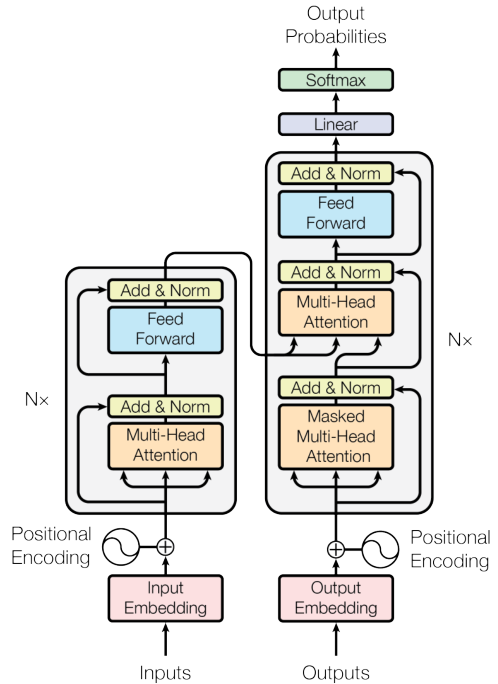
\includegraphics[scale=0.35]{abb/transformer-figure.png}
  \end{center}
  \caption{
      entommen aus "Attention Is All You Need"
      \cite{vaswani2023attentionneed}
  }
\end{figure}
\subsubsection{BERT}
Das BERT-Modell \cite{devlin2019bertpretrainingdeepbidirectional}
ist ein wichtiger Meilenstein im NLP-Bereich und kann 
als eines der ersten Large Language Models betrachtet werden.
Das Modell verbessert die Transformer Architektur, 
indem es die Tokenembeddings verbessert, zwei neue Trainingsaufgaben einführt
und ausschließlich Encoder verwendet.
\begin{figure}[H]
  \begin{center}
    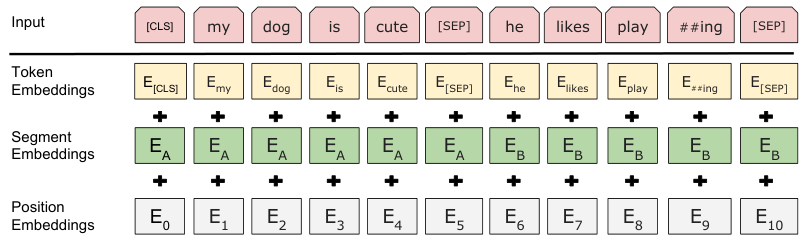
\includegraphics[scale=0.5]{abb/BERT-Tokens.png}
  \end{center}
  \caption{Token Embedding Prozess entnommen aus dem BERT Paper.}
\end{figure}
In Abbildung 2.8 ist der Tokenembedding Prozess abgebildet,
der im Folgenden näher beschrieben wird. Zunächst muss erläutert werden, 
was ein Token ist. Ein Token ist in diesem Fall ein Wort, 
aber generell ist ein Token eine kleinere Zeichenkette, die aus einem 
Text gewonnen wird und einer Bedeutung zugewiesen wird oder in eine 
Zahl umgewandelt wird, um die Weiterverarbeitung zu vereinfachen.\\

Das BERT Modell kombiniert drei unterschiedliche Informationen
in Vektorform, um noch bessere Token Embeddings zu generieren. BERT
verwendet \textit{WordPiece} \cite{wu2016googlesneuralmachinetranslation},
um die Tokenembeddings zu erhalten.
Auf diese werden nun ein Segmentembedding und schließlich die
Positionembeddings addiert. {\bf Segment Embedding} codiert die Information,
welche Tokens strukturell zusammen gehören (Bspw. ein Satz).
Das {\bf Position Embedding} codiert die sequenzielle Position im Input.\\


Die beiden unterschiedlichen Trainingsaufgaben stellen das wichtigste
Puzzleteil dar. Während der Transformer die Token von links nach rechts
vorhersagt, wird BERT darauf trainiert, Wörter vorherzusagen, die auf
beliebiger Position fehlen. Dadurch erhält das Modell Zugang zu dem
Kontext, der sich links und rechts vom zu prädizierenden Token befindet.
Wu et al. benennen diese Trainingsform {\bf Masked Language Modeling}.
Bei diesem Verfahren werden $15 \%$ der Input-Token entweder durch das
\verb|[Mask]| Token oder durch einen zufälligen anderen Token ersetzt.
Dabei werden $10 \%$ der Token, die maskiert werden sollten,
unverändert bleiben. Weitere $10 \%$ werden durch ein zufälliges anderes
Token ersetzt, während die restlichen $80 \%$ durch das \verb|[Mask]| Token 
ersetzt werden.
\pagebreak

Die zweite Trainingsaufgabe ist {\bf Next Sentence Prediction} (NSP),
bei dieser Aufgabe muss das BERT Modell bei der Eingabe von zwei Sätzen 
entscheiden, ob diese sequenziell nacheinander kommen oder nicht.
Bei der einen Hälfte der Daten handelt es sich um zwei Sätze, die nacheinander 
auftreten. Bei der anderen Hälfte der Daten handelt es sich um zufällige,
nicht sequenzielle Sätze. Zur Vorhersage, ob die Sätze nacheinander kommen 
oder nicht, wird das konstante \verb|[cls]| Tokenembedding verwendet, 
welches beim Input immer an erster Stelle steht. Der erste Outputvektor 
ist dann das Ergebnis des \verb|[cls]| Tokens und wird verwendet, um den Output
\verb|isNext| oder \verb|notNext| zu produzieren.\\

Nach dem Training erhält man aus BERT für jeden Inputvektor genau einen 
Outputvektor, diesen kann man dann mit wenig Aufwand weiter verwenden,
um das Modell für bestimmte Probleme in NLP anzupassen 
(engl. fine tuning).

\subsubsection{Sentence Transformer}
Das Sentence-BERT \cite{reimers2019sentencebertsentenceembeddingsusing}
Modell ist der aktuelle Stand der Technik im semantischen Codieren von 
natürlicher Sprache in einem Vektorraum. Die Implementierung der Autoren
ist unter dem Namen \textit{SentenceTransformer} bekannt. Die Motivation 
hinter Sentence-BERT (SBERT) ist das effiziente semantische Vergleichen 
von zwei Sätzen. Wenn man mit BERT herausfinden möchte, wie semantisch
ähnlich zwei gegebene Sätze sind, dann muss man beide Sätze als Input 
in das Modell eingeben. Das heißt, wenn man die Ähnlichkeit von allen
$n$ Sätzen jeweils zueinander haben will, gibt es $\frac{n(n-1)}{2}$ 
Eingaben in das BERT Modell, die man tätigen müsste.
Bei SBERT kann dagegen jeder Satz einzeln eingegeben werden und der
resultierende Output ist dann ein semantischer Vektorraum, indem jeder 
Satz einen semantischen Vektor besitzt. Um die semantische Ähnlichkeit 
zwischen zwei Vektoren zu erhalten, müssen beide Vektoren lediglich in 
eine zu wählende Metrik eingesetzt werden. 
%wird die Kosinus-Ähnilichkeit verwendet: Sei $u,v \in \mathbb{R}^n$, dann setze
%\[
%  Kos(u,v) := cos(\phi) = \frac{u \cdot v}{\|u\|\|v\|} 
%  = \frac
%  {
%    \sum_{i=1}^n u_iv_i
%  }
%  {
%    \sqrt{\sum_{i=1}^n u_i^2} \sqrt{\sum_{i=1}^n v_i^2}
%  }.
%\]
Dies ermöglicht es, die semantische Ähnlichkeit zwischen zwei Vektoren 
effizient zu berechnen.\\

Die Modellarchitektur von SBERT wird als {\bf Siamese Neural Network }
bezeichnet, da zwei unterschiedliche BERT-Modelle verwendet werden,
um beide Sätze in einen Vektor umzuwandeln, aber beide Modelle teilen 
sich die Gewichte.
\pagebreak

\begin{figure}[H]
  \begin{center}
    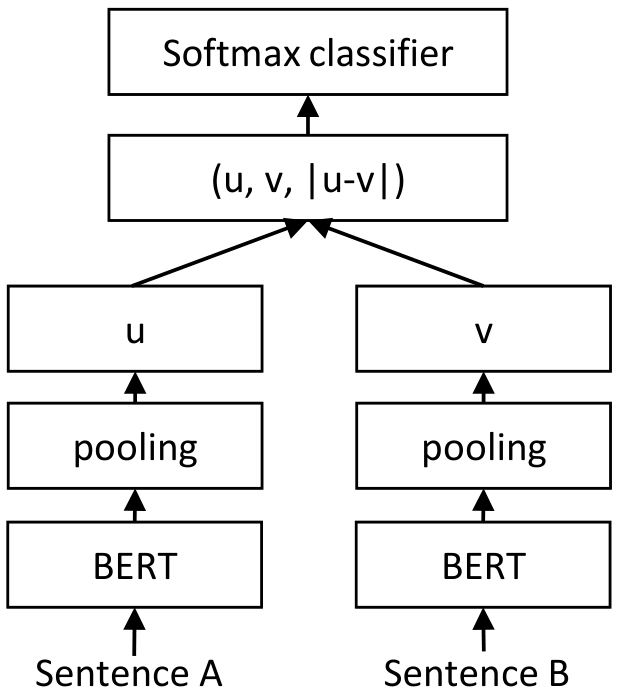
\includegraphics[scale=0.3]{abb/SBERT.png}
  \end{center}
  \caption{SBERT Architektur entnommen aus dem SBERT Paper.}
\end{figure}
In Abbildung 2.9 ist die SBERT Architektur dargestellt, 
in der sich beide BERT Modelle dieselben Gewichte teilen. 
Danach geht der Output von BERT in ein pooling Modul. 
{\bf Pooling} ist das Transformieren von Output mit vielen Vektoren 
in eine geringere Anzahl von Vektoren oder Dimensionen. In diesem Fall 
werden die $n$ Output-Vektoren von BERT in einen einzigen Output-Vektor 
transformiert. Das Default pooling ist der Mittelwert, d.h. auf alle 
Output-Vektoren von BERT wird das arithmetische Mittel angewendet.
Daraus erhält man einen Vektor mit den jeweiligen gemittelten 
BERT-Output-Vektoren.\\

Das BERT Modell wird an die spezielle Aufgabe 
angepasst, zwei Vektoren semantisch zu vergleichen. 
Dafür wird der SNLI Datensatz verwendet, dieser beinhaltet immer 
zwei Sätze und eins von drei möglichen Labels: 
\verb|contradiction|, \verb|neutral|, und \verb|entailment|.
SBERT muss für zwei Sätze vorhersagen, ob sie sich inhaltlich widersprechen,
neutral zueinander sind oder ob der eine Satz eine Fortsetzung des 
anderen ist. Daraus lernt das Modell, ein semantisches Verständnis 
für Sätze zu erlangen. Zur Ermittlung der Labelvorhersage werden die 
jeweiligen Vektoren und ihre Differenz konkateniert. Anschließend 
werden diese mit einem lernbaren Gewicht multipliziert, sodass ein 
Vektor mit drei Dimensionen entsteht. Danach wird der Softmax auf das
Ergebnis angewendet. Die Position in dem Vektor mit dem höchsten Wert 
wird schließlich dem zugehörigen Label zugeordnet. Mathematisch:
Sei $W \in \mathbb{R}^{n\times 3}$ das lernbare Gewicht und 
$v \in \mathbb{R}^n$ Outputvektor von dem pooling, dann
\[
  o = \text{softmax}(Wv).
\]
Nachdem Training bei der Inferenz wird der Vektor, nachdem pooling 
als Output-Vektor ausgeben. SBERT liefert uns also ein Tool, 
um Sätze semantisch in einem Vektorraum abzubilden,
welches sich in späteren Kapiteln als sehr hilfreich herausstellt.
\pagebreak
\subsection{Code Llama}
Die \textit{Code Llama} Familie an Large Language Models wurde von 
Rozière et al. bei Meta AI im Jahre 2024 entwickelt
\cite{rozière2024codellamaopenfoundation}.
{\bf Large Language Models} sind Modelle, die auf
einer großen Menge von Daten trainiert wurden, welche sich darin
auszeichnen, natürliche Sprache verstehen sowie generieren zu
können und deswegen in der Lage sind, eine Vielzahl von Aufgabe
n im NLP-Bereich zu lösen.\\

Meta AI optimiert das vorangegangene Llama2 Modell auf
Programmiersprachen spezifische Aufgaben. Das LLama2 Model wird,
um zum resultierenden Code-llama zu kommen, erneut auf einem neuen
Datensatz trainiert. Dieser besteht aus drei verschiedenen 
Kategorien von Daten. Der größte Teil im Datensatz, mit $85 \%$,
ist mit Programmiersprachen spezifischen Aufgaben verbunden,
indem das Modell darauf trainiert wird, fehlende Programmzeilen in 
einer vergebenen Lücke zu füllen. Dabei kann es sich um Programmcode,
aber auch um Kommentare handeln. Der zweitgrößte Teil im Datensatz,
mit $8 \%$, besteht aus natürlicher Sprache, in der es um 
Programmcode geht. Dieser Teil beinhaltet Diskussion über Quellcode
sowie Fragen und Antworten, welche sich auf Quellcode beziehen. 
Der kleinste Teil im Datensatz mit $7 \%$ besteht aus beliebiger 
natürlicher Sprache, damit das Modell seine alten Fähigkeiten erhält. \\

Das LLama2 Modell ist eine Verbesserung des Llama1 Modells.
Dieses wurde auf neueren Daten trainiert und verwendet einen 
$40 \%$ größeren Datensatz. Zudem wurde die maximale Anzahl 
der gleichzeitig zu verarbeitenden Token verdoppelt. Außerdem 
gab es eine Veränderung in der Llama1 Transformer Architektur. 
In den Attention Modulen werden zwei Werte, die normalerweise 
jedes Mal wieder berechnet werden, geteilt, was bedeutet, dass 
jedes Attention Modul Zugriff auf die gleichen Werte hat.
Dies führt zu geringfügig schlechteren Ergebnissen, jedoch zu
einer deutlichen Leistungssteigerung.\\

Das Llama1 Modell wiederum besteht aus einer Decoder-Only
Transformer Architektur. Der {\bf Decoder-Only} Transformer
besteht lediglich aus Decoder Transformer Blöcken,
wie der Name bereits vermuten lässt. Bei dieser Architektur
ist der anfängliche Input des Decoders die Eingabe des Nutzers.
Auf diese Eingabe wird dann immer wieder das neu generierte Token
drauf konkateniert. Auf diese Weise wird die Eingabe nicht explizit
von dem bereits generierten getrennt, sondern beides wird als 
gleicher Kontext verwendet.\\

Das Besondere an Llama1 ist, dass es nur auf frei verfügbaren
Daten trainiert wurde und dass das Modell Open Source ist. Der
Datensatz besteht aus {\bf English Common Crawl [$67\%$]},
{\bf C4 [$15\%$]}, {\bf Github [$4.5\%$]},
{\bf Wikipedia [$4.5\%$]}, {\bf Gutenberg and Books3 [$4.5\%$]}, 
{\bf ArXiv [$2.5\%$]}, und {\bf Stack Exchange [$2\%$]}.\\

Code Llama ist eine Open Source Software, die unter allen 
verfügbaren Modellen am besten in multilingualen Benchmarks 
abschneidet. Multilingual bedeutet die Verwendung mehrerer 
Programmiersprachen. Diese Eigenschaften machen es sehr geeignet
für diese Arbeit.
\subsection{Code2Vec}
\textit{Code2Vec} ist eine im Jahre 2018 von Alon et al. 
entwickelte Modellarchitektur, die Quellcode in einen semantischen 
Vektor kodiert
\cite{alon2018code2veclearningdistributedrepresentations}.
Nach den Erfolgen in NLP, natürliche Sprache 
in semantische Vektoren zu kodieren, entstand der Wunsch, auch 
Quellcode in semantischen Vektoren abzubilden. Mit diesen Vektoren 
können dann wieder viele verschiedene Aufgaben gelöst werden.
Das motivierende Beispiel im Code2Vec Paper ist die Vorhersage 
eines sinnvollen Namens für eine Funktion. Die Architektur, welche 
in Abbildung 2.10 dargestellt ist, wird im Folgenden erläutert. 
\begin{figure}[H]
  \begin{center}
    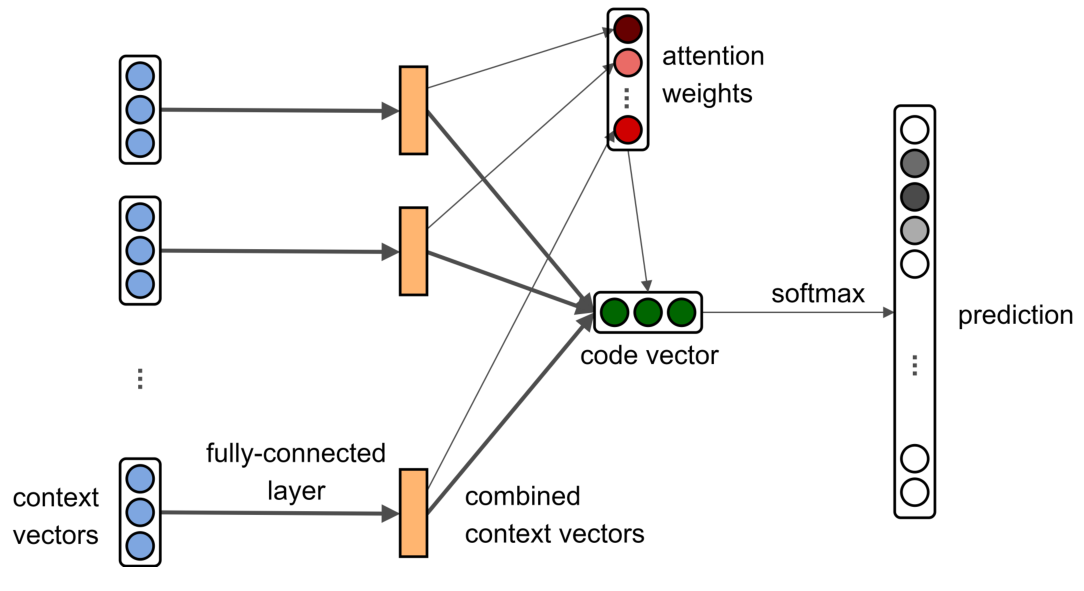
\includegraphics[scale=0.3]{abb/code2vec.png}
  \end{center}
  \caption{
    Code2Vec Architektur entnommen aus dem Code2Vec Paper
    \cite{alon2018code2veclearningdistributedrepresentations}
  }
\end{figure}
Alon et al. fanden heraus, dass eine geeignete Darstellung
von Quellcode als ein mathematisches Objekt ein abstrakter 
Syntaxbaum ist. Dieser erhält die strukturellen Zusammenhänge
zwischen den Tokens und kann gut in einen Vektor kodiert werden.
Die Inputvektoren (context vectors) bestehen jeweils aus einem
Pfad im abstrakten Syntaxbaum, mit dem jeweiligen Starttoken und
Endtoken des Pfades. Danach folgt ein Hidden-Layer, mit \verb|tanh|
als Aktivierungsfunktion. Der endgültige Vektor wird als lineare 
Kombination aus den Outputvektoren und den attention weights 
berechnet. Sei $h_1, \dots, h_n \in \mathbb{R}^d$ die Outputvektoren 
von dem Hidden-Layer
und $\alpha \in \mathbb{R}^n$ der attention weights Vektor.
\[
  \verb| code vector | v = \sum_{i = 1}^n \alpha_i \cdot h_i
\]
Mit dem \verb|code vector| kann dann das gewünschte Label vorhergesagt werden.
Das Modell kann demnach darauf trainiert werden ein bestimmtes Label 
vorherzusagen, welches zu einen Quellcode, also einer reihe an 
\verb |context vector| zugerodnet wird. Nachdem Training kann es dann auch 
Label für Quellcode vorhersagen die es noch nie gesehen hat.\\
Die Trainingsart ist demnach Überwachteslernen, was eine aufbereitung der 
Daten benötigt. Das Modell kann deswegen auch nur Label vorhersagen in der
Inferenz, die es vorher im Training gesehen hat.
\subsection{t-SNE}
{\bf t}-Distributed {\bf S}tochastic {\bf N}eigbor {\bf E}mbedding ({\bf t-SNE})
ist ein Algorithmus, welcher zum visualisieren von hochdimensionalen Daten 
eingesetzt wird. Um das zu ermöglichen reduziert t-SNE die Dimension von 
$n \in \mathbb{N}$ zu einer niedrigeren Dimension wie zwei oder drei, inder
der Mensch die Datenpunkte leicht interpretieren kann, ohne die 
Nachbarschaftsverhältnisse der Datenpunkte in mitleidenschaft zu ziehen.\\
Im folgende wird der Algorithmus skizziert und danach wird aufgezeigt was bei 
der effektiven verwendung von t-SNE zu beachten ist. Die hochdimensionalen 
Datenpunkte werden mit $\mathbf{H}$ und die niedrigdimensionale Datenpukte mit
$\mathbf{N}$ bezeichnet. Der erste schritt des Algorithmuses ist es 
jedem Datenpunktpaar im Datensatz $\mathbf{H}$ ein Ähnlichkeitsscore zu zuweisen.
Dieser wird berechnet indem man zuerst die euklidische Distanz von jeden Datenpaar
berechnet und dann das Ergebnis in eine Wahrscheinlichkeitsverteilung eingibt,
dadurch wird der Wert unter anderen Normalisiert. Das Ergebis ist dann eine 
Tabelle mit einen Ähnlichkeitsscore für jedes Datenpaar in $\mathbf{H}$. Als
nächstes werden die Datenpunkte zufällig in der niedrigen Dimension 
$\mathbf{N}$ angeordnet. Die nachfolgenden zwei schritte werden $T\in \mathbb{N}$
mal wiederholt, wobei $T$ ein Parameter ist der wählbar ist.
\begin{enumerate}
  \item Berechne Ähnlichkeitsscore von $\mathbf{N}$, diesmal wird aber die
      studentische t-Verteilung als wahrscheinlichkeitsverteilung genommen. 
  \item Verschiebe die Datenpunkte von $\mathbf{N}$ um ein kleinen Wert in
    die Richtung, die den Unterschied der Ähnlichkeitsscores von $\mathbf{H}$
    und $\mathbf{N}$ minimiert.
\end{enumerate}
Nach $T$ wiederholung ist der Ähnlichkeitsscore von $\mathbf{N}$ und $\mathbf{H}$
nahe bei einander, d.h. die Nachbarschaftsverhältniss von $\mathbf{N}$ und 
$\mathbf{H}$ sind nun ähnlich.\\
Mitarbeiter von Google haben untersucht, wie man t-SNE sinvoll anwendet und
welche schlüsse man aus der visualisierung ziehen kann. Sie fanden heraus,
dass die wahl der Parameter für das Ergebnis eine wichtige Rolle spielen.
Die wichtigsten Parameter sind die Iterationen $T\in \mathbb{N}$ und die
Perplexity $P \in \mathbb{N}$. Die {\bf Perplexity} kann intuitiv als schätzung 
für die Anzahl an nahen Nachbarn die jeder Datenpunt hat gesehen werden.
Eine geignete Iteration $T$ kann relative einfach durch ausprobieren 
herausgefunden werden: Falls sich die Datenwolke bei erhöhung von $T$
nicht mehr wirklich verändert, ist die Anzahl der Iteration $T$ gefunden
worden. Eine geeignete Perplexity zu finden ist schwieriger, da wir die
hochdimensionalen Nachbarschaftsbeziehungen meistens nicht kennen. Die Autoren
des t-SNE Paper empfehlen eine Perplexity $P \in \{5,6, \dots, 50\}$. Außerhalb
dieses Bereiches können verschieden ungewollte Phänomene auftreten. Bei $P=2$
haben die Google Mitarbeiter herausgefunden das t-SNE bei einer zufällig generierten
Datenwolke, fälschlicher weise kleine Gruppierungen (Cluster) bildet. Falls
$P$ größer ist als die Anzahl der Datenpunkte, ist das Ergebnis überhaupt nicht
interpretierbar. Es ist also immer Sinvoll, mehere Werte für $P$ aus zuprobieren,
um sicher zu gehen das t-SNE keine falschen Nachbarschaftsbeziehungen darstellt.
Die Mitarbeiter von Google fanden ausßerdem heraus, dass sowie die Information 
der Breite eines Clusters, als auch der Abstände von einen Cluster zu einen anderen 
durch t-SNE komplett verloren gehen. Es kann also nach betrachten der
t-SNE Ausgabe keine Aussage über den Durchmesser eines Clusters, die Position
des Cluster und die Lagebeziehungen zwischen Clustern getroffen werden. \\
Der t-SNE Algorithums ist ein wichtiges Tool um qualitative Aussagen über 
Daten zu treffen. Allerdings sollten immer mehrere Parameter ausprobiert werden.
Es kann nur eine Aussage über die existenz von Cluster getroffen werden und 
nicht über ihre geometrischen gegebenheiten. Wenn diese Rahmenbedingungen 
beachtet werden ist t-SNE ein sehr mächtiges visualisierung Tool um eine 
intuition von der Anordnung der Datenpunkte zu erhalten.
% effective use paper: 
% https://distill.pub/2016/misread-tsne/?_ga=2.135835192.888864733.1531353600-1779571267.1531353600
%pgf plots

%\subsection{Stand der Technik} in Introduction
% Self supervised learning (JTrans, PalmTree)
% Same Source policy (Safe)
%  Clap
\section{Methodik}
\subsection{Datensatz}
Im Maschinellen lernen hat der Datensatz bzw. die Trainingsdaten den
größten Einfluss auf die güte des Modells. Wir haben die 
Open Source Standard C Bibliothek von GNU ausgewählt.
Die Sprache C wurde gewählt, da sie die weit verbreiteste zu 
maschienen Code kompellierbare Sprache ist. Die GNU Bibliothek 
wurde zum einen ausgewählt, da
die Qualität des Quellcodes hoch ist, das liegt daran das das Projekt 
seit 1987 existiert 
und die große Community jederzeit auf Fehler im Quellcode aufmerksam
machen kann. Zum anderen wird die Bibliothek weitgehend in vielen
Applikationen eingesetzt. Der wohl wichtigste Punkt ist, dass
man mit diesen Datensatz die Ergebnisse gut vergleichen kann, denn
die C Bibliothek ist im posix standard festgelet und wurde mehrmals
unterschiedlich implementiert, dadurch erhält man mehrer hoch Qualitative
Quellcode Projekten, die die selbe Semantik aufweisen. Damit kann dann 
bspw. die Binary Code Similarity Detection Aufgabe durchgeführt werden.\\
Die {\bf Binary Code Similarity Detetection} (BCSD) gibt an wie 
unterschiedlich zwei  in Assebler vorliegende Funktionen sind.
Da unterschiedliche implementierungen zu unterschiedlichen 
Assembler Code kompelliert werden, kann mit unterschiedlichen
Standard-C-Bibliotheken die den POSIX Standard implementieren,
getestet werden, ob das finale Modelle beide implementerungen 
als sehr ähnlich klassifiziert.

% Warum ist die Auswahl des Datensatzes wichtig
% Warum Glibc? 
% Gleicher Standard mit gleicher Semantik unterschiedlich Implementierung
\subsection{Datenpipeline}
Die große praktische Arbeit der Bachelorarbeit war es, eine große Menge
von Daten in verschiedensten Darstellungen immer wieder umzuwandeln. Dabei 
wurde jeder Zwischenschritt gespeichert, damit nicht jede Darstellung immer
wieder generiert werden muss. Im folgenden wird die generelle Architektur 
wie Daten verabeitet werden vorgestellt (engl. Pipeline), um ein Überblick
über den praktischen Teil dieser Arbeit zu geben.
\begin{figure}[H]
  \begin{center}
    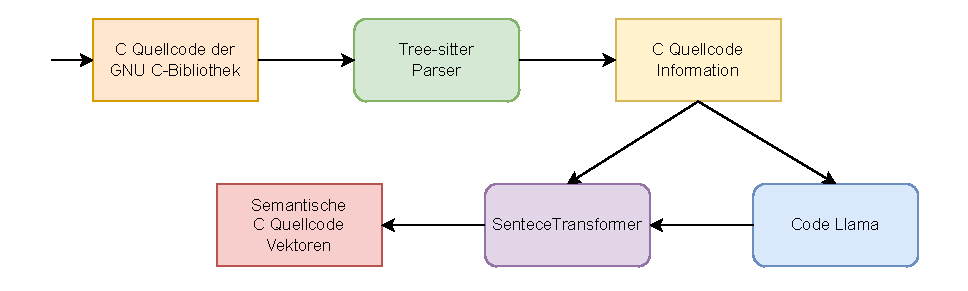
\includegraphics[scale=0.8]{abb/data-pipeline.pdf}
  \end{center}
  \caption{Datenpipeline}
\end{figure}
In der Abbildung 3.1 ist die Datenpipeline dargestellt, dabei sind Vierecke 
mit runden Ecken Tools die Daten in eine andere Darstellung umwandeln und
Vierecke mit spitzen Ecken repräsentieren Darstellungen von Daten. Die erste
Darstellung sind die Rohdaten, das entspricht den unverarbeiteten C Quellcode
aus der GNU Standard C Bibliothek. Nun brauche wir aber nicht alle Teile des
Quellcode sondern nur bestimmeteile, zum Beispiel arbeiten wir nur mit Funktionen
d.h. alle Datenstrukturen die in dem Quellcode definiert werden, wollen wir
aus dem Quellcode entfernen. Die Zerlegung und Umwandlung des Inputs 
in sinvolle Teile wird parsing genannt. In dieser Arbeit wurde {\bf Tree-sitter}
als Parser verwendet, welcher alle populären Programmiersprachen in Syntaxbäume
umwandeln kann. Ursprünglich wurde Tree-sitter für den Texteditor Atom entwickelt
und wird heute noch in vielen Texteditoren für bspw. Syntaxhighliting verwendet.
Generell kann Tree-sitter jedoch für alles das Quellcode verarbeiten will 
verwendet werden. Aus dem Syntaxbaum kann dann jeglich gewünschte Information 
entnommen werden. Diese Quellinformationen werden dann estmal zwischen gespeichert,
damit von nun an, die verabeitung hier angesetzt werden kann. Die Quellinforamtionen
beziehen sich immer auf eine Funktion, also ist das Format eine Tabelle die
für jede Funktion in den Rohdaten die gewünschten Quellinforamtionen enthält.
Danach gibt es eine Abzweigung, entweder werden die Quellinformationen Code Llama
nochmal erklärt und dann in den SentenceTransformer gegeben oder die 
Quellinformation wird direkt in den SentenceTransformer gegeben. Schließlich 
erhält man wieder eine Tabelle die gespeichert wird, die für jede Funktion
das zugewisene Semantische Embedding enthält. Bei dieser Architektur kann
mühelos jedes Tool ausgewechselt werden solange die Ausgabeformate eingehalten
werden.
% Treesitter erklären
% Source Code information in json datei speichern
% Dann Source code information in Vektor umwandeln
% Modularität -> Vorteile dieses Designs 
\subsection{Stabilität von SentenceTransformer}
In dem vorherigen unterkapitel haben wir gesehen das der finale schritt 
für alle Daten der SentenceTransformer ist, deswegen ist er das Herzstück
der Datenpipeline. In dieser Arbeit sollen verschiedene semantische 
beschreibungen des Quellcodes in natürlicher Sprache verglichen werden.
Um hier sinvoll zu messe, müssen ,wie bei einem physikilischen Experiment,
alle anderen Elemente in der Datenpipeline konstante Ergebnisse liefern und 
nicht schwanken. Aus diesen Gründen wird im folgenden Untersucht, wie stabil
sich der SentenceTransformer bei selber Eingabe verhält. Im optimafall 
sollte der SentenceTransfomer bei selben Input selbes Ergebnis liefern. \\
Um das zu überprüfen wurden $n = ?$ Code-llama Quellcode Erklärungen 
$m = ?$ mal in den Sentence Transformer eingegeben, dabei beträgt der 
höchste Abstand von zwei Vektoren die aus der gleichen Erklärung resutliert
sind $d = ?$. Dieser Abstand ist hinreichend gerin um ihn in der Evaluation
zu vernachlässigen. Der Sentence Transformer ist also für die Anwendung in
dieser Arbeit hinreichend Stabil.





% Label Prozess sollte stabil sein bzw. deterministisch, sonst
% kann keine aussage über die Güte der Labels getätig werden
% Tabelle mit Ergebnissen der standardabweichungen

\
\section{Funktionskommentare}
\subsection{Motivation}
Bevor ein Programm kompelliert wird und nur noch die nötigsten Informationen
für den Computer bestehen bleiben, gibt es eine Menge an Informationen die 
die Semantik der Funktion in natürlicher Sprache beschreiben. Eine offensichtliche
Quellcodeinformation die im optimalfall die Semantik der Funktion in natürlicher
Sprache beschreibt ist der Kommentar. Ein gelungener Kommentar für eine Funktion
beschreibt präzise die kernfunktion der Prozedur, d.h. der Input, den Output
und wie diese umwandlung erfolgt. Dieser könnte man dann mit dem 
SentenceTransformer in einen Semantischen Vektoraum abbilden, was in einen
Semantischen Quellcode Vektor resultiert.
% Warum könnten funktionskommentare dafür geignet sein die Semantik einer
% Funktion zu beschreiben
\subsection{Methodik} 
Das parsen der Kommentare wurde wie in dem Unterkapitel Datenpipeline erwähnt 
mit Tree-sitter realisiert. Dabei gab es zwei große Designentscheidungen zu treffen.
Zum einen welche Kommentare in einer Funktion berücksichtigt werden sollen und
zweitens was macht man mit Funktionen die eine leicht Variationen von einer
anderen Funktion sind und deswegen keine Kommentare besitzten. Ein gutes Beispiel
für das zweite Problem ist \verb|exit| und \verb|__run_exit_handlers|, wenn
\verb|exit| aufgerufen wir, ruft diese Funktion einfach 
\verb|__run_exit_handlers| mit speziellen Parametern auf. Dabei ist \verb|exit|
nicht kommentiert, aber \verb|__run_exit_handlers| ist kommentiert.\\
{\color{red} Bei der ersten Designentscheidung welche Kommentare ich berücksichtige,
habe ich mich ausschließlich für den Kommentar direkt über der Funktion 
entschieden, da die einzeiligen Kommentare in der Funktion meistens keinen
großen Semantischen Wert haben, sondern auf gefahren oder Designentscheidungen
 hinweisen. (Beleg maybe: A survey on Reasearh of code comment)} Für das zweite Problem habe ich mich für folgende Lösung entschieden.
Falls eine Funktion keinen Kommentar besitzt, dann werden die Kommentare von
allen Funktionen die in den Funktionskörper aufgerufen werden konkatiniert und
als eigenen Kommentar übernommen. Dardurch hat \verb|exit| dann einen Kommentar
und zwar exakt den selben wir \verb|__run_exit_handlers|.\\
Hierbei muss man aufpassen das der Prozess des parsens nicht zu speziell an
den vorliegenden Daten angepasst wird, sonst verliert er seine Allgemeingültigkeit.
Deswegen habe ich mich nicht auf weitere Optimierungen die ein wenig mehr Kommentare
erbrignen könnten eingelassen, sondern es bei den oben beschriebenen belassen.
% Probleme beim Parsen, wo sucht man nach Kommentaren?
% Keine einheitliche Konvention
% -> Unterschiedliche Code Base Unterschiedliche Kommentar Konventionen
\section{Code2Vec}
\subsection{Motivation} 
Das besondere an Code2Vec ist, dass es den Quellcode in eine abstrakten
Syntaxbaum kodiert. Damit nutzt Code2Vec alle Quellcodeinformationen die
in dem Quellcode vorhanden sind. Danach wird das Modell darauf trainiert
eine Eigenschaft in natürlicher Sprache über den Quellcode vorherzusagen.
Bei dieser herangehensweise wird also kein SentenceTransformer verwendent
sondern der Semantische Vektroraum wird durch Training des Code2Vec Modells
als Nebenprodukt erzeugt. Wie in den Paper wird auch hier Code2Vec
darauf trainiert Funktionsnamen vorherzusagen. Die Implementierung des Code2Vec
Modells wurde von den Autorn nur auf Java trainiert, deswegen gab es
einige anpassungen nötig, um Code2Vec auf C Quellcode trainieren zu können.
Da das Code2Vec Modell auf überwachtes Lernen basiert, muss der Datensatz 
vor dem Training erstmal aus den ursprünlgichen Quellcode aufbereitet werden.
% Warum könnte code2vec semantisch gute Vektoren produzieren
\subsection{Adaption auf C}
Um das Cod2Vec Modell Trainineren zu können muss aus den rohen Quellcode einer
Funktion jeweils ein abstrakter Syntaxbaum und den Funktionsnamen extrahiert 
werden. Die Autoren des Papers stellen ein Tool für Java zu verfügung, welches
die Extrahierung von abstrakten Syntaxbäumen und Funktionsnamen aus Java Quellcode
ermöglicht.\\
Der \textit{astminer} von JetBrains stellt ermöglicht es aus C-Quellcode 
abstrakte Syntaxbäume und Funktionsnamen zu extrahieren. Das
Tool wurde von dem JetBrains Research Team entwickelt, 
um Quellcode in abstrakte Syntaxbäume (AST) zu kodieren, 
welche sich als Inputformat für maschinelle Lernen Modelle eignen. \\
Das Cod2Vec Modell braucht ein bestimmtes Format indem der Datensatz vorliegen
muss. Ein Trainingsbeispiel besteht jeweils aus einen Funktionsnamen, dem
Label und einer Liste von Kontexten, welche
den AST repräsnetieren sollen. Ein Kontext besteht aus einen Token gefolgt von
einer Pfadbeschreibung zu einen anderen Token, welches danach folgt.
Dieses Code2Vec Format kann durch eine zusätzlich Option in der Konfiguration
des astminers generiert werden. Trotz dieser Option die mit "code2vec" betitelt
ist, ist der Output von dem \textit{astminer} nicht direkt von Code2vec
verwendbar. Das Tool weist nämlich jeden Token eine einzigartige Zahl zu und
verwendet dann in Datensatz nur noch die Zahl. Dieses Format reduziert zwar
den Speicheraufwand stark, aber es wird von Code2vec nicht als valide Eingabe
akzeptiert. Demnach mussten noch die Nummern wieder zu der passenden Token
umgewandelt werden.
\begin{figure}[H]
  \begin{center}
    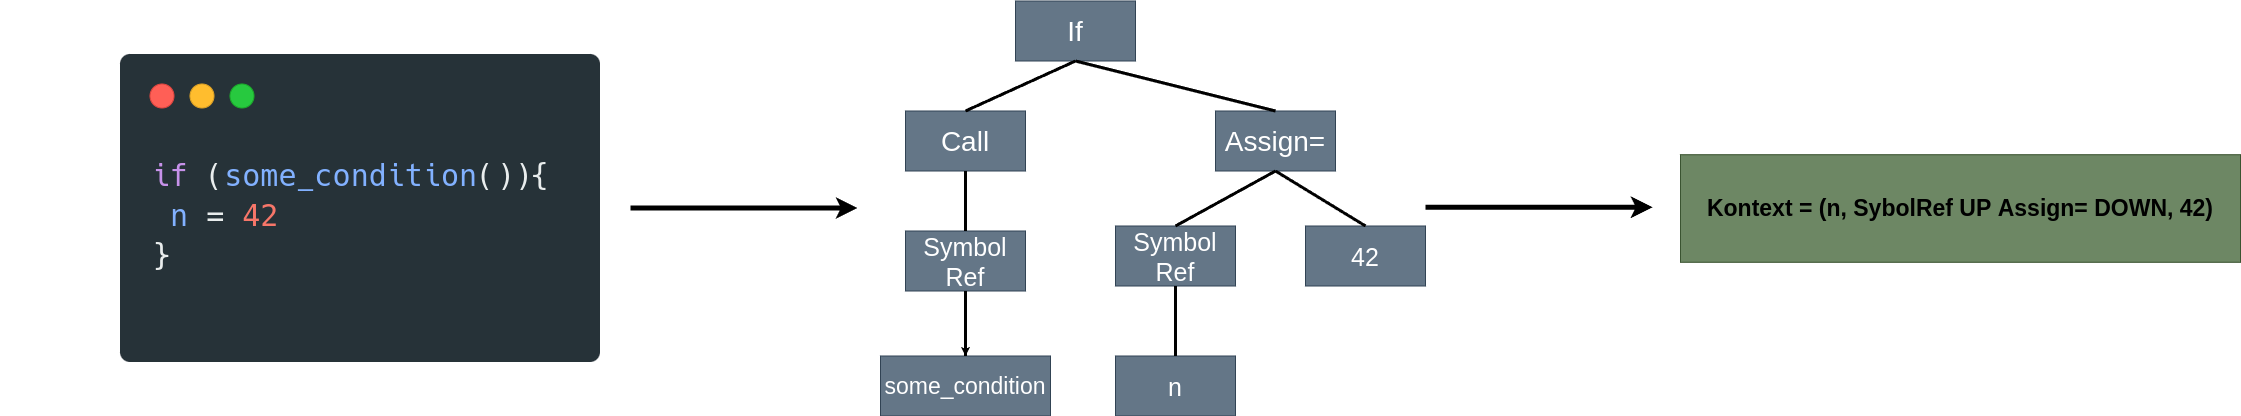
\includegraphics[scale=0.2]{abb/ast-extraction-example.drawio.png}
  \end{center}
  \caption{Extrahierung eines Kontexts}
\end{figure}
Da es unterschiedliche Koventionen für Funktionsnamen gibt, wie Bspw. Camelcase und
Snakecase, normalisert der \textit{astminer} die Funktionsnamen. Dadurch sind
die Trainingsdaten unabhängig von den spezifischen Quellcodekonventionen.
\begin{example}
  \hfill
  \begin{center}
    Snakecase: \verb|funktions_name| $\to$ {\bf funktions\text{\textbar}name } \\
    Camelcase: \verb|funktionsName| $\to$ {\bf funktions\text{\textbar}name}
  \end{center}
\end{example}
Code2Vec kann nach dem Training für jede Funktion einen Hochdimensionalen
Vektor ausgeben, der die Semantik der Funktion beschreiben soll. Damit Code2Vec
diesen Vektor generiert, muss der abstrakte Syntaxbaum eingegeben werden. Die
abstrakten Syntaxbäume können nur durch ihren normalisierten Namen identifiziert
werden, da sie als Tupel in dieser Form im Datensatz vorliegen.
Die normalisierten Namen können aber nicht mehr eindeutig dem initialen
Namen zugeordnet werden,da bei der Normalisierung Informationen verloren
gehen. Um jedoch Cod2Vec mit anderen Ansätzen wie Funktionskommentaren 
vergleichen zu können, müssen die normalisierten Namen wieder zu den
ursprünglichen Namen zurückgeführt werden. Aufgrund dessen mussten im
Quellcode von astminer änderungen vorgenommen werden, so dass zu jeder 
Position eines Trainingsbeispiels im Datensatz den ursprünglichen 
Funktionsnamen zugeordnet werden konnte. \\
Mit diesen Anpassungen die noch zusammen gefügt werden mussten konnte nun
Trainiert werden und nach Abschlusses des Trainings konnten die semantischen
Vektoren, durch diese Anpassungen verglichen und ausgewertet werden.
% Code ändern bei astminer um die Namen der Funktionen am ende zuzordnen zu können
% da die Namen normalisiert werden und nicht mehr eindeutig zugeordnet werden können
% code2vec erklären
\subsection{Training}
Das Ziel beim Training war es die selbe Qualität wie im Paper zu erhalten.
Also die selben Ergebnisse für Java auch für C-Quellcode zu replizieren.
Für den Anwendungszweck einen Datensatz zu erstellen der für eine Funktion
in Assemblersprache einen semantischen Vektor als Label zuordnet, können
bestimmte problemstellungen beim generellen trainieren von Modellen 
ignoriert werden. Eine Problemstellung bei Modellen ist es inwiefern
das Modell generalisiert, also wie Leistungsfähig das Modell auf
neuen Daten im gegensatz zu den Trainingsdaten ist. Diese Problemstellung
muss nicht beachtet werden, da das Ergebnis kein fähiges Modell ist, sondern
semantische Vektoren. Auch der kleine Datensatz mit $n = 5155$ Datenpunkten,
ist zwar für die Güte des Modells problematisch, jedoch nicht für die
resultierenden semantischen Vektoren. Selbst wenn das Modell nur die 
passenden Funktionsnamen auswendig lernt, enstehen dabei Vektoren die
gewisse Inforamtionen des Namens wiederspiegeln. Nachdem das Trainingsszeneario
genau das selbe wie im Paper ist, wurden alle Trainingsparameter gleich gelassen.
Die Ergebnisse nach der 84 Epoche sind: {\bf Precision: $65.6$, F1: $65.1$, 
Recall: $64.7$}. Diese Werte sind etwas über den Werten von den Code2Vec 
Autoren, sie kamen beim Full Test Set auf : {\bf Precision: $63.1$, F1: $58.4$, 
Recall: $54.4$}. Dabei ist hervorzuheben das unser Test und Trainings Datensatz
der selbe ist, im gegensatz zu dem Test Datensatz von Code2Vec. Die vorgehensweise
ist normalerweise ein grober Fehler, da wir nicht die Generalisierung des 
Modells messen. In diesem speziellen Anwedungszweck ist jedoch die Güte des
Modell nicht von bedeutung, sondern nur die die güte der Erzeugten Vektoren.
Diese werden von der Verwendung des gleichen Datensatzes beim Testen nicht in
mitleidenschaft gezogen. \\
Damit haben wir ähnliche Ergebnisse wie aus dem Paper und können diese mit
den anderen vorgestellten Ansätzen vergleichen.
%Parameterwahl und Ergebnisse
% Ganzes engeneering und pain hinter code2vec
\section{Funktionsnamen}
Eine andere Quellinformation, die in jedem Quellcode enthalten ist,
sind die Funktionsnamen. 
Funktionsnamen sollen in wenigen Wörtern den Kerninhalt der Funktion
wiederspiegeln. %function names.pdf
Dadurch eignen sich Funktionsnamen um die Semantik einer Funktion 
zu beschreiben. Außerdem ist die Extrahierung der Funktionsnamen
keine schwierige Aufgabe. Hierfür wäre Tree-sitter nicht unbedingt
nötig, aber falls ein Datensatz für eine andere Sprache wie Rust
erstellt werden sollte, müsste der Parser jedes mal angepasst werden.
Deswegen wurde hier für die einfache Erweiterung des Programms,
Tree-sitter verwendet. Tree-sitter bietet nämlich Parser für eine
große Anzahl an Sprachen an.
% Motivation warum es gute semantische Vektoren erzeugen konnte
% Parsen
% Eigentlich einfach aber wenn man in Zukunft 
% Viele System nahe sprachen dazu nehmen will
% wie Rust, C, Zig, usw. 
% Ist es doch schwieriger
% -> Treesitter
\section{Coddelama-Erklärungen}
\subsection{Motivation}
Large Language Models werden immer besser Quellcode selbst zuschreiben,
zu verstehen und zusammen zu fassen. Eine Zusammenfassung von Quellcode
in natürlcher Sprache spiegelt die Semantik des Quellcodes wieder. So ist
auch Code-Llama fähig Quellcode zu erklären und somit einen Text zu generieren
der die Semantik der Funktion enthält. Dieser Ansatz verwendet wie Code2Vec
jede Quellcodeinforamtion, da der gesamte Quellcode als Eingabe genutzt wird.
Da wir einen Datensatz erstellen sollte der Labelgenerierugnsprozess 
deterministisch sein, das ist Code-llama anfänglich nicht. Außerdem ist der
Eingabetext in Code-llama, abgesehen von dem Quellcode, entscheidend für die 
Erklärungen.

% Warum LLM's gute Embeddings produzieren könnten.
% Wir erzeugen uns eine zusammenfassung vom code
% "optimale" Kommentare
% Was ist Codellama und warum benutzten wir es?
\subsection{Methodik}
Die Quellcode erklärungen werden von Code-Llama erzeugt, indem Code-Llama
eine präzise Fragestellung und den gesamten Quellcode einer Funktion enthält.
Die Fragestellung wurde aus dem Clap Projekt übernommen, diese haben sich
auch damit beschäftigt, wie die Fragestellung formulliert werden muss
um Semantik reiche und präzise Quellcodeerklärungen zu erhalten. \\
Damit
der Code-Llama Output deterministisch ist, muss der Temperatur Parameter
auf Null gesetzt werden. Der Parameter ist Teil einer Zufalls komponente
bei der Auswahl des nächstens Tokens, ist dieser auf Null wird der Token
mit der höchsten Score gewählt, dieser bleibt bei gleicher Eingabe immer
der selbe. Leider ist der Detminismus trotzdem nicht garantiert, wie die
studio von ... heraus fand. Der Grund ist laut ... das bei denen vielen
fließkomma operationen rundungsfehler enstehen. Diese Erkentnisse stammen
aber aus einen anderen Anwendungszweck.\\
Die Stabilität mit Temperatur Null sollte deswegen für den Anwendungszweck
dieser Arbeit getestet werden.
Um das zu überprüfen wurden von $n = ?$ Funktionen der Quellcode mit Fragestellung
$m = ?$ mal in Code-Llama eingegeben, bei den resultierenden Vektoren beträgt der 
höchste Abstand von zwei Vektoren die aus der gleichen Quellcode resutliert
sind $d = ?$. Dieser Abstand ist wieder hinreichend gering um ihn in der Evaluation
zu vernachlässigen. Das Code-llama LLM ist also für die Anwendung in
dieser Arbeit hinreichend Stabil.
% Vorgehensweise
% Von Chatbot zu relativ deterministischen Modell
% Ergebnisse der Standardabweichung mit Temperatur 0
\section{Ergebnisse}
\subsection{Evaluierung durch Experten}
\subsubsection{Methodik}
% Aufbau des Fragebogens und
% Stichproben Größe, vlt. Vorstellung der Experten
\subsubsection{Auswertung und Ergebnisse}
% Diskussion der Ergebnisse
% Folgerungen das CodeLlamma "gute" Embeddings produziert 
\subsection{Qualitative Evaluierung} 
% t-SNE Plots
% Vielleicht nochmal subsections mit Funktionsname, Funktionskommentare, 
% Funktionserklärung, und Code2Vec Vektoren
% Probleme des jeweiligen Ansatzes mit drei Vektoren
\subsection{Quantitative Evaluierung} 
% Formel um zwei Embedding spaces zu vergleichen
% Formel erklären und rechtfertigen
% Aus Umfrage rechtfertigen Codellama Summaries als gute
% embeddings zu verwenden
\section{Limitation}
\section{Diskussion}
%copy Evaluation
% Zusammenfassung der jeweiligen Resultate
% Funktionnamen -> Nicht geignet, da zu wenig informationen und abkürzungen
% Funktionskommentare -> Je nach Projekt geignet, aber nicht allgemeingültig
%     deswegen eher ungeignet
% Code2Vec -> Kommt nur knapp an mit benutzuten Daten an Names ran also nicht 
% geignet
\section{Fazit}
\section{Results: Comparing natural language supervised methods for creating Rich Binary Labels}
\begin{itemize}
  \item Stabilität von Sentence Transformer
  \item Kommentare von Funktionen um Embeddings zu generieren
  \item Funktionsnamen von Funktionen um Embeddings zu generieren
  \item Code2Vec um Embeddings zu generieren
  \item CodeLlama Erklärungen von Funktionen um Embeddings zu generieren
  \item Evaluierung durch tSNE-Plots
  \item Evaluierung durch Experten
  \item Evaluierung durch Formel
\end{itemize}
$ I_{k}: \mathbf{N} \times \mathbf{N} \times \mathbf{N}^{k} \to [0,1]$
\[ I_{k}(x,i,v) = \begin{cases*} 
      1 & , $\exists j \in \mathbf{N}: x = v_j \land i = j$  \\
      \frac{1}{2} & , $\exists j \in \mathbf{N}: x = v_j \land i \neq j$\\
      0   & , \text{otherwise}
                \end{cases*} \]
$E_k: \nat^k \times \nat^k \to [0,1]$
\[ E_k(u,v) = \frac{1}{G_k} \sum^{k}_{i=1} \frac{I_k(u_i,i,v_i)}{log_2(i+1)}\]
wo $G_k := \sum_{i=1}^{k} \frac{1}{log_2(i+1)}$.\\\\
$CMP_k: \mathbf{R}^{N\times l} \times \mathbf{R}^{N\times l} \times 
\{ \mathbf{R}^l \times \mathbf{R}^{N\times l} \to \mathbf{N}^k \} 
\times \{ \mathcal{P}([0,1]) \to [0,1] \} \to [0,1]$

\[ CMP_k(X,Y,f_k,agg) = agg(\{E_k(f_k(X_{i,j},X),f_k(Y_{i,j},Y)) | j \in \{1,2,3, \dots N\}\})\]


\section{Conclusion}

\pagebreak

\section{General Addenda}

If there are several additions you want to add, but they do not fit into the thesis itself, they belong here.

\subsection{Detailed Addition}

Even sections are possible, but usually only used for several elements in, e.g.\ tables, images, etc.

\section{Figures}
\subsection{Example 1}
\subsection{Example 2}


\pagebreak

\microtypesetup{protrusion=false}
\listoffigures{}
\listoftables{}
\microtypesetup{protrusion=true}

\clearpage
\printglossaries

\pagebreak

\addcontentsline{toc}{section}{Literatur}
\pagestyle{fancy}

\bibliographystyle{IEEEtran}
\bibliography{bibliography} %bib-filename

\nocite{*} %List all bib-entries

\end{document}
